%
% projektion.tex
%
% (c) 2018 Prof Dr Andreas Müller, Hochschule Rapperswil
%
\documentclass[tikz,12pt]{standalone}
\usepackage{times}
\usepackage{amsmath}
\usepackage{txfonts}
\usepackage[utf8]{inputenc}
\usepackage{graphics}
\usetikzlibrary{arrows,intersections,math}
\begin{document}

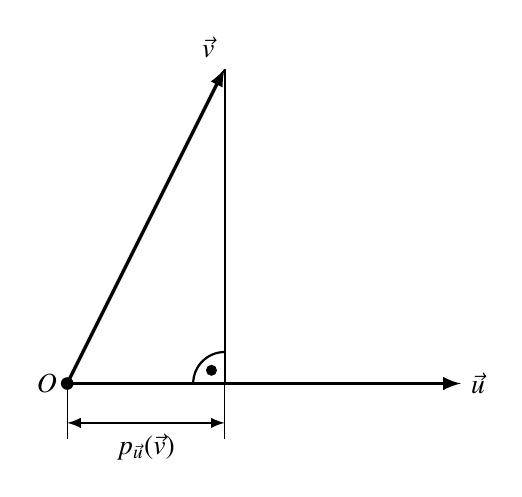
\begin{tikzpicture}[>=latex,thick]

% Nullpunkt
\node at (0,0) [left] {$O$};
\fill (0,0) circle[radius=0.08];

% Vektor u
\draw[->,line width=1.2pt] (0,0)--(5,0);
\node at (5,0) [right] {$\vec{u}$};

% Vektor v
\draw[->,line width=1.2pt] (0,0)--(2,4);
\node at (2,4) [above left] {$\vec{v}$};

% Projektion
\draw[line width=0.8pt] (2,0)--(2,4);
\def\r{0.4}
\draw (2,\r) arc (90:180:\r);
\fill ({2-0.42*\r},{0.42*\r}) circle[radius=0.07];

% Bemassung
\draw[line width=0.5pt] (0,0)--(0,-0.7);
\draw[line width=0.5pt] (2,0)--(2,-0.7);
\draw[<->, line width=0.7pt] (0,-0.5)--(2,-0.5);
\node at (1,-0.5) [below] {$p_{\vec{u}}(\vec{v})$};

\end{tikzpicture}

\end{document}

